\documentclass[Softwaredesign/Softwaredesign_main.tex]{subfiles}

\begin{document}

\textbf{Display design}
\begin{figure}[H]
    \centering
    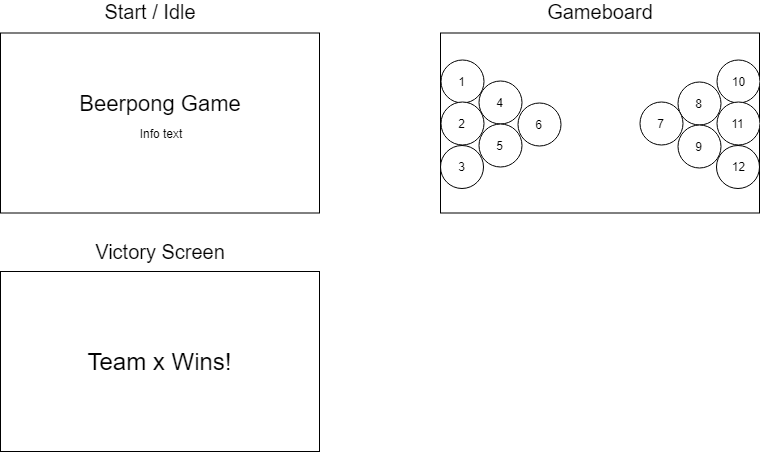
\includegraphics[scale=0.5]{Softwaredesign/GUI/Pictures/Boards.png}
    \caption{Forskellige design af "Game boards". Der ses: en IDLE state,  En Gameboard state,  en Victory screen og en Service screen. Hvad der definere en "state", er  at  de har en unik baggrund. Det vil sige at teksten vist på skærmen f.eks. hold navne  ikke ændre på hvilken state man befinder sig i.  }
    \label{gameboards}
\end{figure}

På figur \ref{gameboards} kan ses forskellige states som displayet kan vise.  Der er et ''Start/Idle'' state. Dette er det state som displayet vil vise når der intet spil er igangværende. Gamboard state er det state som er aktivt når et spil er igangværende. Victory screen er det state som aktiveres når et hold rammer den sidste kop,  og spillet er vundet. Service state er det state som er aktivt hvis der er mindre en to bolde tilbage i \textbf{Balldispenser}. \\
Måden der skiftes mellem states er via. beskeder fra en message queue; for at se mere omkring message queue se ??.  De beskeder håndteres så af en af masse "handler funktioner", som styre hvad der vises på skærmen; for mere omkring de omtalte handlers se afsnit  \fullref{swdesign:sec:display_q} \\
Der laves et Statemachine diagram på figur \ref{GuiDisplayStatemachine}, som viser sammenhængen mellem de tilgængelig states  og de omtalte handlers.


\begin{figure}[H]
    \centering
    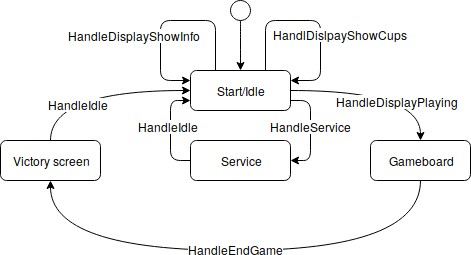
\includegraphics[scale=0.8]{Softwaredesign/GUI/Pictures/Gui_displaystatemachine.png}
    \caption{Statemachine for display tilstand}
    \label{GuiDisplayStatemachine}
\end{figure}


\end{document}